\documentclass{beamer}
\usepackage{graphicx}
\title{My Introduction}
\author{Nathan Ma}
\date{2024/11/03}

\begin{document}

\begin{frame}
  \titlepage
\end{frame}

\begin{frame}{Biography}
  \begin{itemize}
    \item \textbf{Birthday:} Aug 31, 1998
    \item \textbf{Hometown:} Tong Chuan, Xi'an, China
    \item \textbf{Program:} Plant Breeding and Genetics
    \item \textbf{Expected Graduation:} May, 2025
  \end{itemize}
\end{frame}

\begin{frame}{Favorite Animal}
  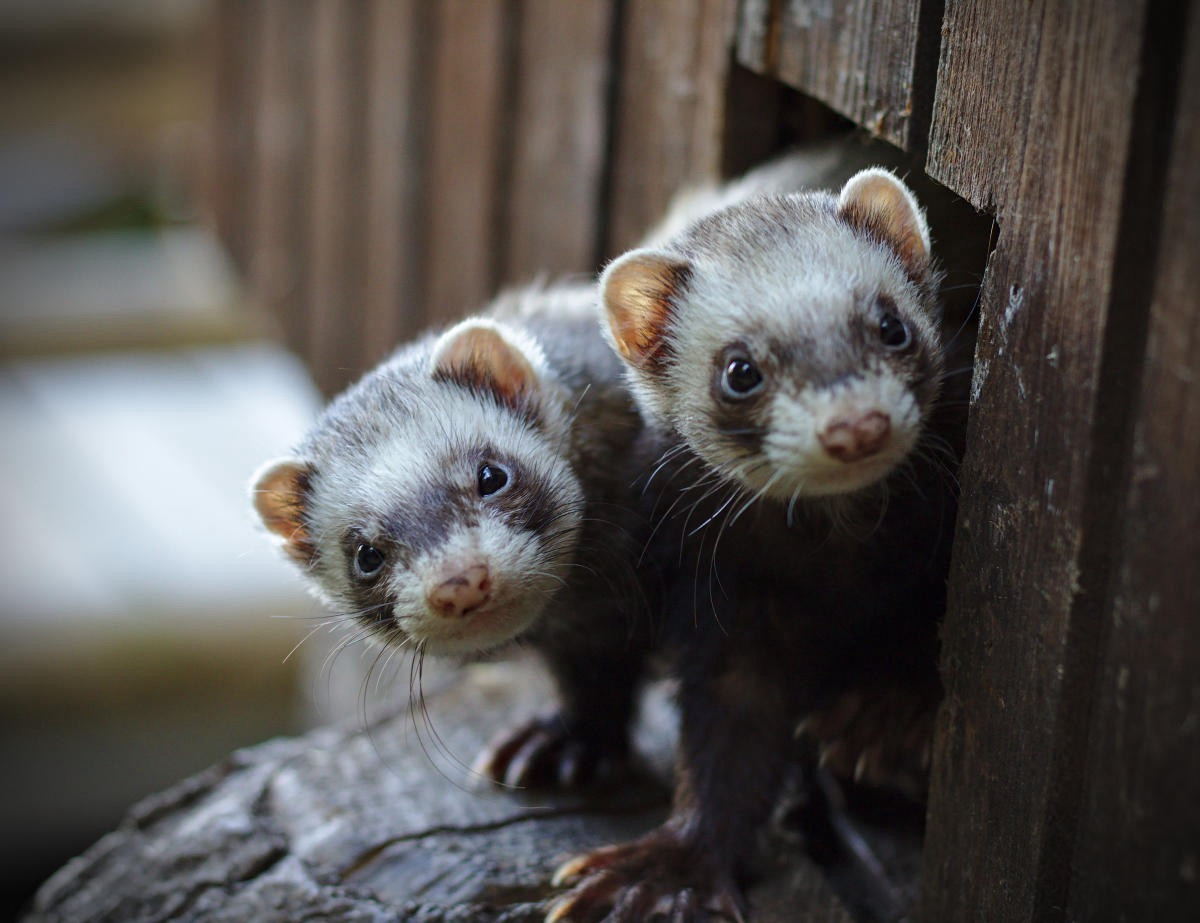
\includegraphics[width=\textwidth]{./animal.jpg}
\end{frame}

\begin{frame}{My Favorite Plot}
<<echo=FALSE, message=FALSE, fig=TRUE>>=
library(ggplot2)
library(tidyverse)
cookie <- read.csv("./choc_chip_cookie_ingredients.csv", stringsAsFactors = FALSE)
cookie_data <- cookie[, -1]
cookie_data$Ingredient <- as.character(cookie_data$Ingredient)
cookie_data$Text <- as.character(cookie_data$Text)
cookie_data$Recipe_Index <- as.character(cookie_data$Recipe_Index)
cookie_data$Unit <- as.character(cookie_data$Unit)
cookie_data$Rating <- as.numeric(cookie_data$Rating)
cookie_data$Quantity <- as.numeric(cookie_data$Quantity)

ingredient_count <- cookie_data %>%
  group_by(Ingredient) %>%
  summarise(Recipe_Count = n_distinct(Recipe_Index)) %>%
  mutate(Total_Recipes = n_distinct(cookie_data$Recipe_Index),
         Proportion = Recipe_Count / Total_Recipes) %>%
  arrange(desc(Recipe_Count)) %>%
  slice(1:20)

ingredient_count %>%
  ggplot(aes(x = reorder(Ingredient, Proportion), y = Proportion)) +
  geom_bar(stat = "identity", fill = "steelblue") +
  coord_flip() +
  labs(title = "Proportion of Recipes Containing Each Ingredient (Top 20)",
       x = "Ingredient",
       y = "Proportion of Recipes") +
  theme_minimal()
@
\end{frame}

\begin{frame}{My CV}
  \begin{itemize}
    \item [CV Link:] \url{https://www.overleaf.com/read/zhwgtwcrvdfj#dc3a51}
  \end{itemize}
\end{frame}


\end{document}
